\chapter{Programas de control del sistema de espectroscopia Kerr} \label{AppKerrAuto}
\section{Adquisición continua}
\begin{figure}[!hbt]
	\centering
	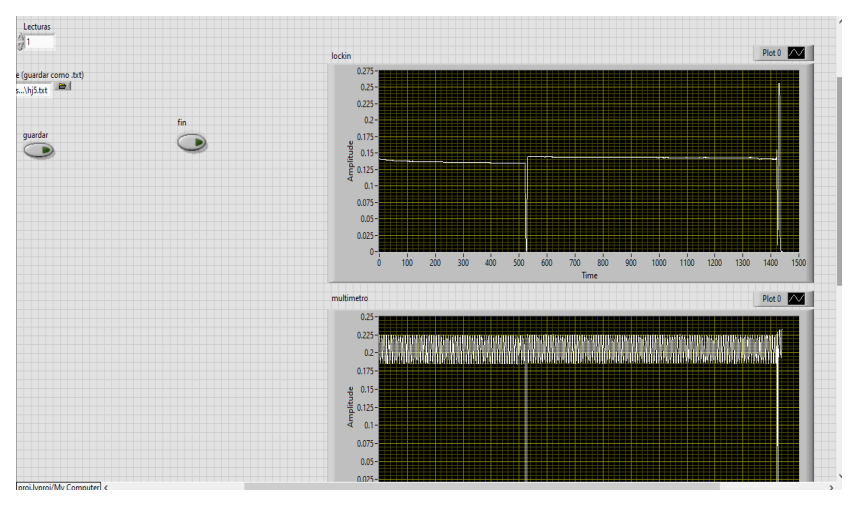
\epsfig{file=fiApLB/continuo.eps, scale=0.8}
	\caption[Interfaz gr\'afica del software utilizado para verificar la se\~nal.]{Software para verificar que si se tenga respuesta de efecto Kerr. }
	\label{Lab:fig:continuo}
\end{figure} 
En la figura \ref{Lab:fig:continuo} se muestra la interfaz gr\'afica de este programa que es utilizado para verificar que se obtiene respuesta de efecto Kerr magneto-\'optico en la muestra, este software simplemente est\'a leyendo los datos que reciben el lock in y el mult\'imetro y se grafican estos dos datos y la divisi\'on entre ellos  con respecto al tiempo y el usuario var\'ia la corriente en las bobinas para variar el campo magn\'etico externo que se aplica en la muestra y se puede observar el cambio en la se\~nal. Este programa permite promediar varias lecturas de estos dispositivos adem\'as de que puede guardar los dados en en un archivo de texto si es que el usuario as\'i lo desea.

\section{Programa para medici\'on de hist\'eresis}
En la figura \ref{Lab:fig:mk} se muestra la interfaz gr\'afica del programa utilizado para obtener el ciclo de hist\'eresis, la cual permite al usuario definir el rango en el que se medir\'a la hist\'eresis, fijar el n\'umero de lecturas que se considerar\'an en esta medici\'on y asignar un nombre al archivo de texto en donde se guardar\'a la informaci\'on. Adem\'as muestra al usuario las gr\'aficas de la se\~nal que adquiere del mult\'imetro digital y el amplificador lock in en funci\'on del campo externo aplicado, as\'i mismo muestra la divisi\'on entre la e\~nal obtenida de estos dos aparatos. Para obtener la hist\'eresis del \'angulo ($\theta_k$) y elipticidad ($\eta_k$) Kerr es necesario realizar una medici\'on con el lock in sintonizado a $f$ y otra a $2f$ con el fin de resolver el sistema de ecuaciones formado por las expresiones \ref{Met:ec:divI1} y \ref{Met:ec:divI2}. 
\begin{figure}[!hbt]
	\centering
	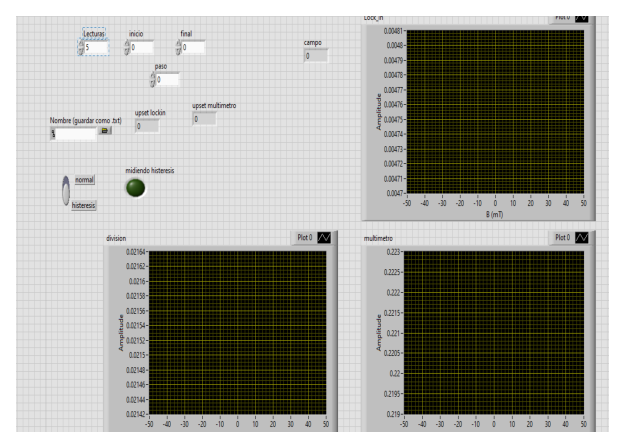
\epsfig{file=fiApLB/mk.eps, scale=1.1}
	\caption[Interfaz gr\'afica del software utilizado para obtener la hist\'eresis.]{Software para obtener la hist\'eresis. }
	\label{Lab:fig:mk}
\end{figure}
\section{Programa para adquirir el espectro Kerr}
  
\begin{figure}[!hbt]
	\centering
	\subfigure[Configuraci\'on]{
			
\epsfig{file=fiApLB/confEsp.eps, scale=1}
			\label{Lab:fig:conf}
	}
    \subfigure[Medici\'on]{
    	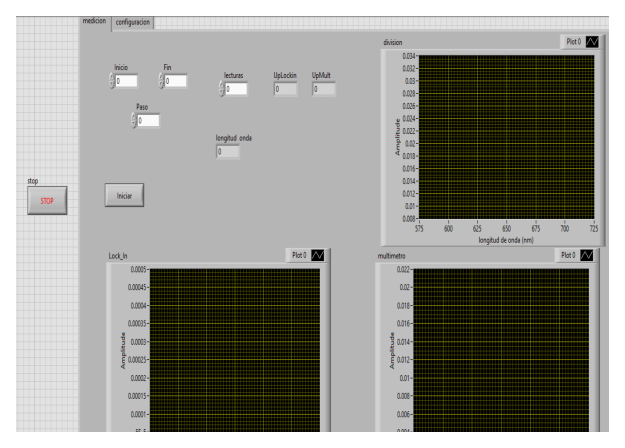
\epsfig{file=fiApLB/medEsp.eps, scale=1}
    	\label{Lab:fig:med}
    }
    \caption[Interfaz gr\'afica del software utilizado para obtener el espectro de efecto Kerr.]{Software para obtener el espectro de efecto Kerr.}
    \label{Lab:fig:esp}
\end{figure}
En la figura \ref{Lab:fig:esp} se muestra la interfaz gr\'afica del programa utilizado para adquirir la se\~nal en funci\'on de la longitud de onda, este programa consta de dos partes; la primera  (Fig. \ref{Lab:fig:conf}) es utilizada para cambiar la longitud de onda del monocromador  y el PEM y la segunda (Fig. \ref{Lab:fig:med}) es utilizada para obtener el espectro, la interfaz gr\'afica permite al usuario introducir los valores de inicio, fin y el cambio de la longitud de onda, adem\'as permite introducir el n\'umero de lecturas y el nombre del  archivo en el que se guardar\'a la informaci\'on, de igual forma que en el caso del programa de adquisici\'on de la hist\'eresis, se utilizan tres gr\'aficas para mostrar los datos que se adquieren el mult\'imetro, el lock in y la divisi\'on entre \'estos.
\endinput